\documentclass[tikz,border=0pt]{standalone}
\usepackage[T1]{fontenc}
\usepackage{libertinus}
\usepackage{tikz}
\usetikzlibrary{calc,positioning,shapes.geometric,fadings}

% Colors - Deep space with multi-colored glowing network
\definecolor{DeepSpace}{RGB}{8,18,32}
\definecolor{MidSpace}{RGB}{15,30,50}
\definecolor{GlowCyan}{RGB}{0,230,200}
\definecolor{GlowTeal}{RGB}{0,190,170}
\definecolor{GlowBlue}{RGB}{70,160,255}
\definecolor{GlowPurple}{RGB}{140,100,220}
\definecolor{GlowPink}{RGB}{230,100,170}
\definecolor{NodeCore}{RGB}{255,255,255}
\definecolor{EdgeGlow}{RGB}{80,200,190}
\definecolor{MetalLight}{RGB}{195,200,212}
\definecolor{MetalDark}{RGB}{130,140,158}

\begin{document}
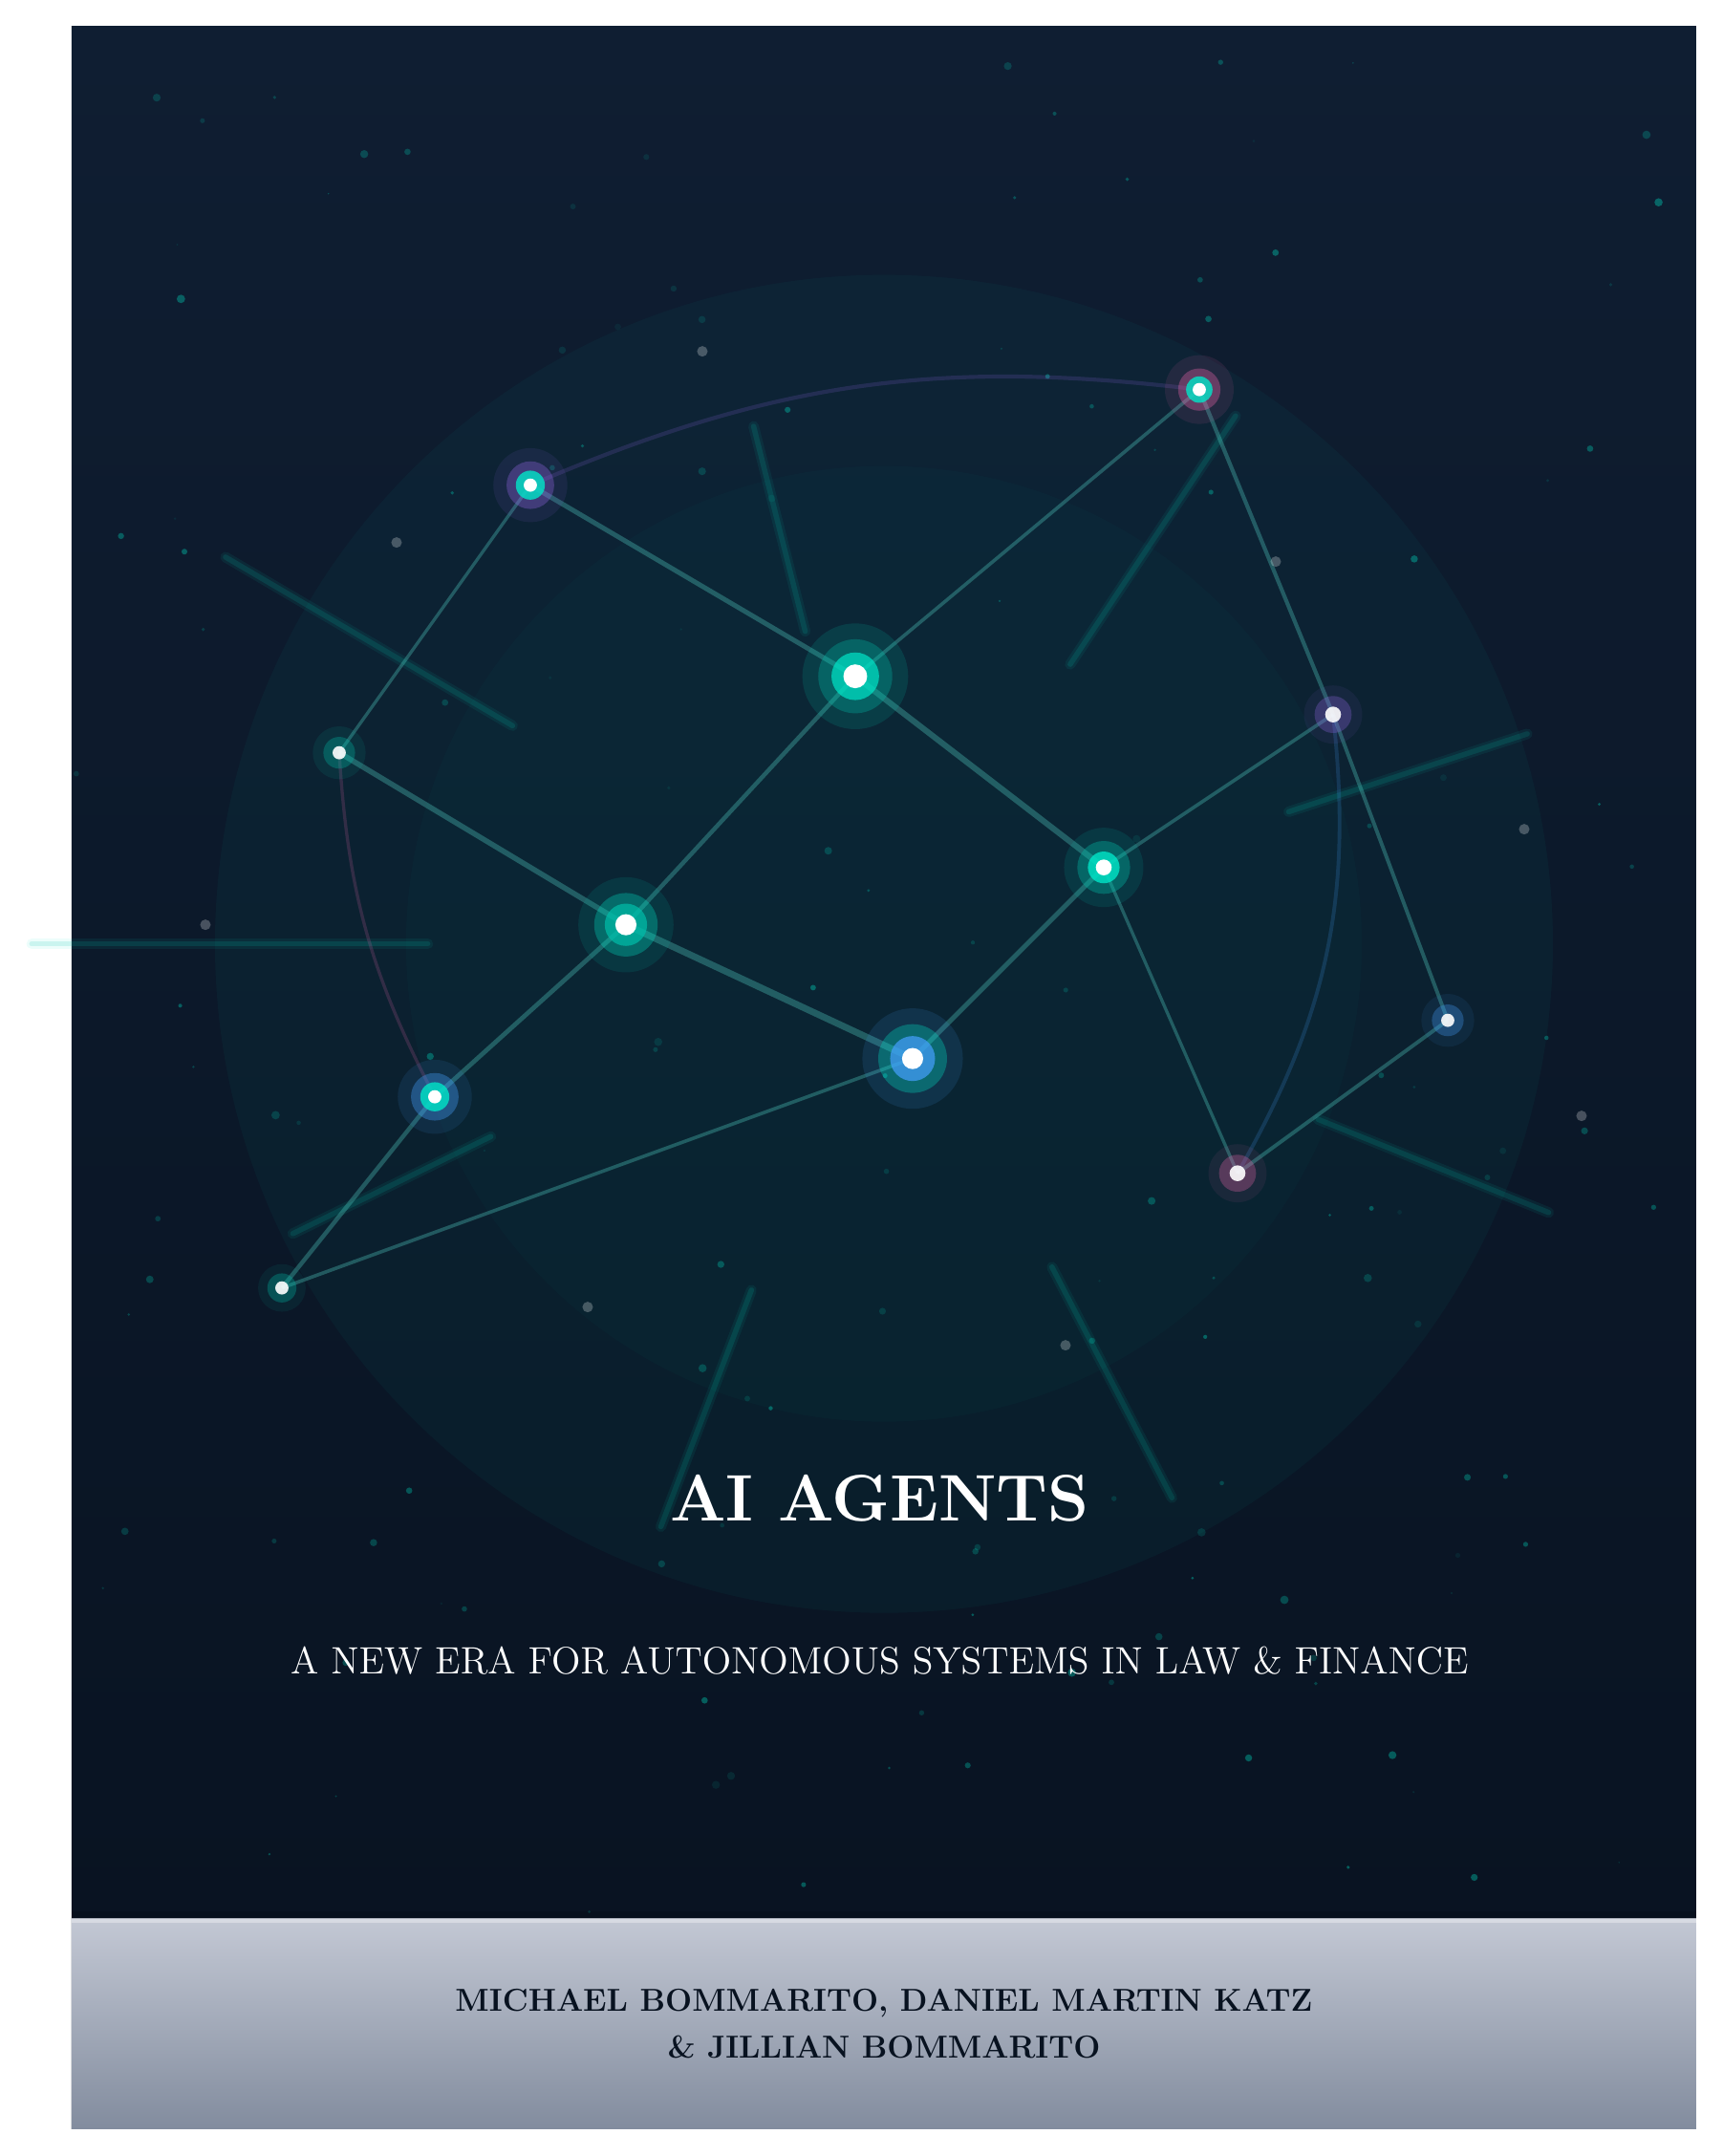
\begin{tikzpicture}

\def\pagewidth{8.5in}
\def\pageheight{11in}

% Background gradient
\shade[top color=MidSpace, bottom color=DeepSpace]
  (0,0) rectangle (\pagewidth,\pageheight);

% Central radial glow
\fill[GlowCyan, opacity=0.04] (4.25in, 6.2in) circle (3.5in);
\fill[GlowTeal, opacity=0.03] (4.25in, 6.2in) circle (2.5in);

% Scattered particles - more of them for depth
\foreach \i in {1,...,150} {
  \pgfmathsetmacro{\px}{random()*8.5}
  \pgfmathsetmacro{\py}{random()*11}
  \pgfmathsetmacro{\psize}{0.3 + random()*1.3}
  \pgfmathsetmacro{\popacity}{0.06 + random()*0.3}
  \fill[GlowCyan, opacity=\popacity] (\px in, \py in) circle (\psize pt);
}

% Motion blur streaks - scattered asymmetrically
\foreach \angle in {25, 65, 100, 140, 180, 215, 255, 290, 330} {
  \pgfmathsetmacro{\len}{1.2 + random()*1.0}
  \pgfmathsetmacro{\startdist}{2.3 + random()*0.4}
  \pgfmathsetmacro{\sx}{4.25 + \startdist*cos(\angle)}
  \pgfmathsetmacro{\sy}{6.2 + \startdist*sin(\angle)*0.7}
  \pgfmathsetmacro{\ex}{4.25 + (\startdist+\len)*cos(\angle)}
  \pgfmathsetmacro{\ey}{6.2 + (\startdist+\len)*sin(\angle)*0.7}
  \draw[GlowTeal, opacity=0.15, line width=2pt, line cap=round]
    (\sx in, \sy in) -- (\ex in, \ey in);
  \draw[GlowCyan, opacity=0.07, line width=4pt, line cap=round]
    (\sx in, \sy in) -- (\ex in, \ey in);
}

% ABSTRACT NETWORK GRAPH
\begin{scope}

  % Define node positions - organic scattered layout
  \coordinate (n1) at (2.4in, 8.6in);
  \coordinate (n2) at (5.9in, 9.1in);
  \coordinate (n3) at (1.4in, 7.2in);
  \coordinate (n4) at (4.1in, 7.6in);
  \coordinate (n5) at (6.6in, 7.4in);
  \coordinate (n6) at (2.9in, 6.3in);
  \coordinate (n7) at (5.4in, 6.6in);
  \coordinate (n8) at (7.2in, 5.8in);
  \coordinate (n9) at (1.9in, 5.4in);
  \coordinate (n10) at (4.4in, 5.6in);
  \coordinate (n11) at (6.1in, 5.0in);
  \coordinate (n12) at (1.1in, 4.4in);

  % ===== EDGE CONNECTIONS (behind nodes) =====
  \begin{scope}[opacity=0.35]
    \draw[EdgeGlow, line width=1.2pt] (n1) -- (n3);
    \draw[EdgeGlow, line width=1.8pt] (n1) -- (n4);
    \draw[EdgeGlow, line width=1.3pt] (n2) -- (n4);
    \draw[EdgeGlow, line width=1.5pt] (n2) -- (n5);
    \draw[EdgeGlow, line width=2pt] (n3) -- (n6);
    \draw[EdgeGlow, line width=1.6pt] (n4) -- (n6);
    \draw[EdgeGlow, line width=2.2pt] (n4) -- (n7);
    \draw[EdgeGlow, line width=1.3pt] (n5) -- (n7);
    \draw[EdgeGlow, line width=1.4pt] (n5) -- (n8);
    \draw[EdgeGlow, line width=1.7pt] (n6) -- (n9);
    \draw[EdgeGlow, line width=2.5pt] (n6) -- (n10);
    \draw[EdgeGlow, line width=1.8pt] (n7) -- (n10);
    \draw[EdgeGlow, line width=1.2pt] (n7) -- (n11);
    \draw[EdgeGlow, line width=1.4pt] (n8) -- (n11);
    \draw[EdgeGlow, line width=1.6pt] (n9) -- (n12);
    \draw[EdgeGlow, line width=1.3pt] (n10) -- (n12);
  \end{scope}

  % Curved accent connections
  \begin{scope}[opacity=0.18]
    \draw[GlowPurple, line width=1.5pt, bend left=15] (n1) to (n2);
    \draw[GlowPink, line width=1.2pt, bend right=12] (n3) to (n9);
    \draw[GlowBlue, line width=1.4pt, bend left=18] (n5) to (n11);
  \end{scope}

  % ===== PRIMARY NODES (largest, brightest) =====
  % Node 4
  \fill[GlowCyan, opacity=0.12] (n4) circle (20pt);
  \fill[GlowTeal, opacity=0.3] (n4) circle (14pt);
  \fill[GlowCyan, opacity=0.7] (n4) circle (9pt);
  \fill[NodeCore] (n4) circle (4.5pt);

  % Node 6
  \fill[GlowTeal, opacity=0.12] (n6) circle (18pt);
  \fill[GlowCyan, opacity=0.3] (n6) circle (12pt);
  \fill[GlowTeal, opacity=0.7] (n6) circle (8pt);
  \fill[NodeCore] (n6) circle (4pt);

  % Node 10
  \fill[GlowBlue, opacity=0.12] (n10) circle (19pt);
  \fill[GlowCyan, opacity=0.3] (n10) circle (13pt);
  \fill[GlowBlue, opacity=0.7] (n10) circle (8.5pt);
  \fill[NodeCore] (n10) circle (4pt);

  % ===== SECONDARY NODES =====
  % Node 1
  \fill[GlowPurple, opacity=0.1] (n1) circle (14pt);
  \fill[GlowPurple, opacity=0.35] (n1) circle (9pt);
  \fill[GlowCyan, opacity=0.8] (n1) circle (5.5pt);
  \fill[NodeCore] (n1) circle (2.5pt);

  % Node 2
  \fill[GlowPink, opacity=0.1] (n2) circle (13pt);
  \fill[GlowPink, opacity=0.35] (n2) circle (8pt);
  \fill[GlowCyan, opacity=0.8] (n2) circle (5pt);
  \fill[NodeCore] (n2) circle (2.5pt);

  % Node 7
  \fill[GlowCyan, opacity=0.1] (n7) circle (15pt);
  \fill[GlowTeal, opacity=0.35] (n7) circle (10pt);
  \fill[GlowCyan, opacity=0.8] (n7) circle (6pt);
  \fill[NodeCore] (n7) circle (3pt);

  % Node 9
  \fill[GlowBlue, opacity=0.1] (n9) circle (14pt);
  \fill[GlowBlue, opacity=0.35] (n9) circle (9pt);
  \fill[GlowCyan, opacity=0.8] (n9) circle (5.5pt);
  \fill[NodeCore] (n9) circle (2.5pt);

  % ===== TERTIARY NODES (smaller) =====
  % Node 3
  \fill[GlowCyan, opacity=0.08] (n3) circle (10pt);
  \fill[GlowTeal, opacity=0.3] (n3) circle (6pt);
  \fill[NodeCore, opacity=0.9] (n3) circle (2.5pt);

  % Node 5
  \fill[GlowPurple, opacity=0.08] (n5) circle (11pt);
  \fill[GlowPurple, opacity=0.3] (n5) circle (7pt);
  \fill[NodeCore, opacity=0.9] (n5) circle (3pt);

  % Node 8
  \fill[GlowBlue, opacity=0.08] (n8) circle (10pt);
  \fill[GlowBlue, opacity=0.3] (n8) circle (6pt);
  \fill[NodeCore, opacity=0.9] (n8) circle (2.5pt);

  % Node 11
  \fill[GlowPink, opacity=0.08] (n11) circle (11pt);
  \fill[GlowPink, opacity=0.3] (n11) circle (7pt);
  \fill[NodeCore, opacity=0.9] (n11) circle (3pt);

  % Node 12
  \fill[GlowTeal, opacity=0.08] (n12) circle (9pt);
  \fill[GlowTeal, opacity=0.3] (n12) circle (5.5pt);
  \fill[NodeCore, opacity=0.9] (n12) circle (2.5pt);

\end{scope}

% Extra floating particles near main graphic
\foreach \x/\y in {1.7/8.3, 3.3/9.3, 6.3/8.2, 0.7/6.3, 7.6/6.8, 2.7/4.3, 5.2/4.1, 7.9/5.3} {
  \fill[NodeCore, opacity=0.25] (\x in, \y in) circle (2pt);
}

% ============ TITLE SECTION ============

\node[anchor=center, align=center] at (4.25in, 3.3in) {
  {\fontsize{48}{56}\selectfont\bfseries\color{white}AI AGENTS}
};

\node[anchor=center, align=center] at (4.25in, 2.45in) {
  {\fontsize{15}{20}\selectfont\color{white!85}A NEW ERA FOR AUTONOMOUS SYSTEMS IN LAW \& FINANCE}
};

% ============ METALLIC BAND ============

\shade[top color=MetalLight, bottom color=MetalDark]
  (0, 0) rectangle (\pagewidth, 1.1in);

\fill[white, opacity=0.35] (0, 1.08in) rectangle (\pagewidth, 1.1in);
\fill[black, opacity=0.12] (0, 1.1in) rectangle (\pagewidth, 1.14in);

\node[anchor=center, align=center] at (4.25in, 0.55in) {
  {\fontsize{13}{16}\selectfont\color{DeepSpace}\textbf{MICHAEL BOMMARITO, DANIEL MARTIN KATZ}}\\[0.08in]
  {\fontsize{13}{16}\selectfont\color{DeepSpace}\textbf{\& JILLIAN BOMMARITO}}
};

\end{tikzpicture}
\end{document}
